\section{Результаты измерений}
Длина струны $l=50\pm 0{,}05\,\text{см}$.

\begin{table}[!ht]
    \centering
    \caption{Частоты основных гармоник, Гц}
    \begin{tabular}{|l|l|l|l|l|l|}
    \hline
        $n$ & $m=1037.988\,\text{г}$ & $m=1375.988\,\text{г}$ & $m=1857.988\,\text{г}$ & $m=2319.688\,\text{г}$ & $m=2820.588\,\text{г}$ \\ \hline
        1 & 133.8 & 154.2 & 176.4 & 196.3 & 217.9 \\ \hline
        2 & 217.07 & 309 & 355.7 & 393.3 & 436.1 \\ \hline
        3 & 408 & 464 & 533.2 & 589.9 & 654.5 \\ \hline
        4 & 544.5 & 619.3 & 711.7 & 786.7 & 872.8 \\ \hline
        5 & 683 & 774.2 & 890.3 & 983.6 & 1091.7 \\ \hline
        6 & 820.1 & 931 & 1069.3 & 1181.1 & 1310.2 \\ \hline
        7 & 956.7 & 1088.7 & 1248.7 & 1379.8 & 1530.1 \\ \hline
        8 & 1096.3 & 1244.8 & 1429.3 & 1578.6 & 1750.2 \\ \hline
        9 & 1239.6 & 1404.3 & 1610.7 & 1778.2 & 1971.5 \\ \hline
    \end{tabular}
\end{table}

\begin{figure}[ht!]
    \centering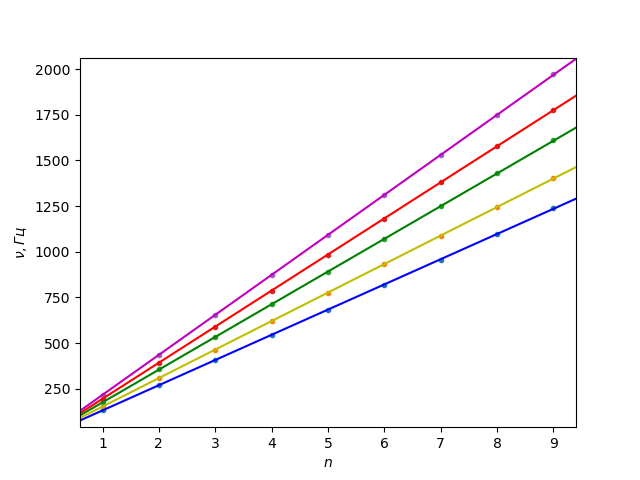
\includegraphics[width=0.8\linewidth]{img/plt1.png}
\end{figure}

\begin{gather*}
    v_1=138.0\pm0{,}4\,\text{м}/\text{с}\\
    v_2=156.1\pm0{,}4\,\text{м}/\text{с}\\
    v_3=179.1\pm0{,}4\,\text{м}/\text{с}\\
    v_4=197.6\pm0{,}4\,\text{м}/\text{с}\\
    v_5=219.0\pm0{,}4\,\text{м}/\text{с}\\
\end{gather*}

\begin{figure}[ht!]
    \centering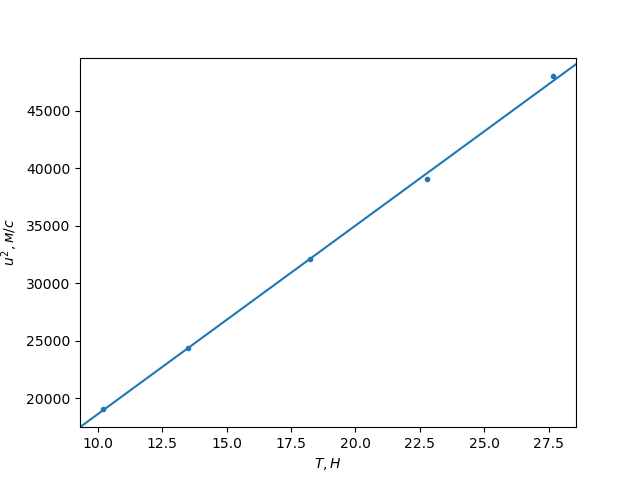
\includegraphics[width=0.8\linewidth]{img/plt2.png}
\end{figure}

\[\rho = 564\pm 2\,\text{мг}/\text{м}\]

Почти совпадает с значением, указаным на установке ($568{,}4\,\text{мг}/\text{м}$)

\begin{table}[!ht]
    \centering
    \caption{Частоты основных гармоник, Гц}
    \begin{tabular}{|l|l|l|l|l|l|}
    \hline
        $n$ & $\nu_1,\text{Гц}$ & $\nu_2,\text{Гц}$ & $\nu_3,\text{Гц}$ \\ \hline
        1 & 217.773 & 217.703 & 217.876 \\ \hline
        2 & 198.11 & 198.09 & 198.24 \\ \hline
        3 & 177.026 & 176.976 & 177.116 \\ \hline
    \end{tabular}
\end{table}

\begin{gather*}
    Q_1=1258\\
    Q_2=1320\\
    Q_3=1264\\
    Q\approx 1280
\end{gather*}

Благодаря высокой добротности струны, возможно возбуждение колебаний при кратных частотах
генератора, меньших частоты первой гармоники. При частоте генератора $\nu=108.95\,\text{Гц}$.
На экране осциллографа можно увидеть фигуру Лиссажу с одним самопересечением.

\begin{figure}[ht!]
    \centering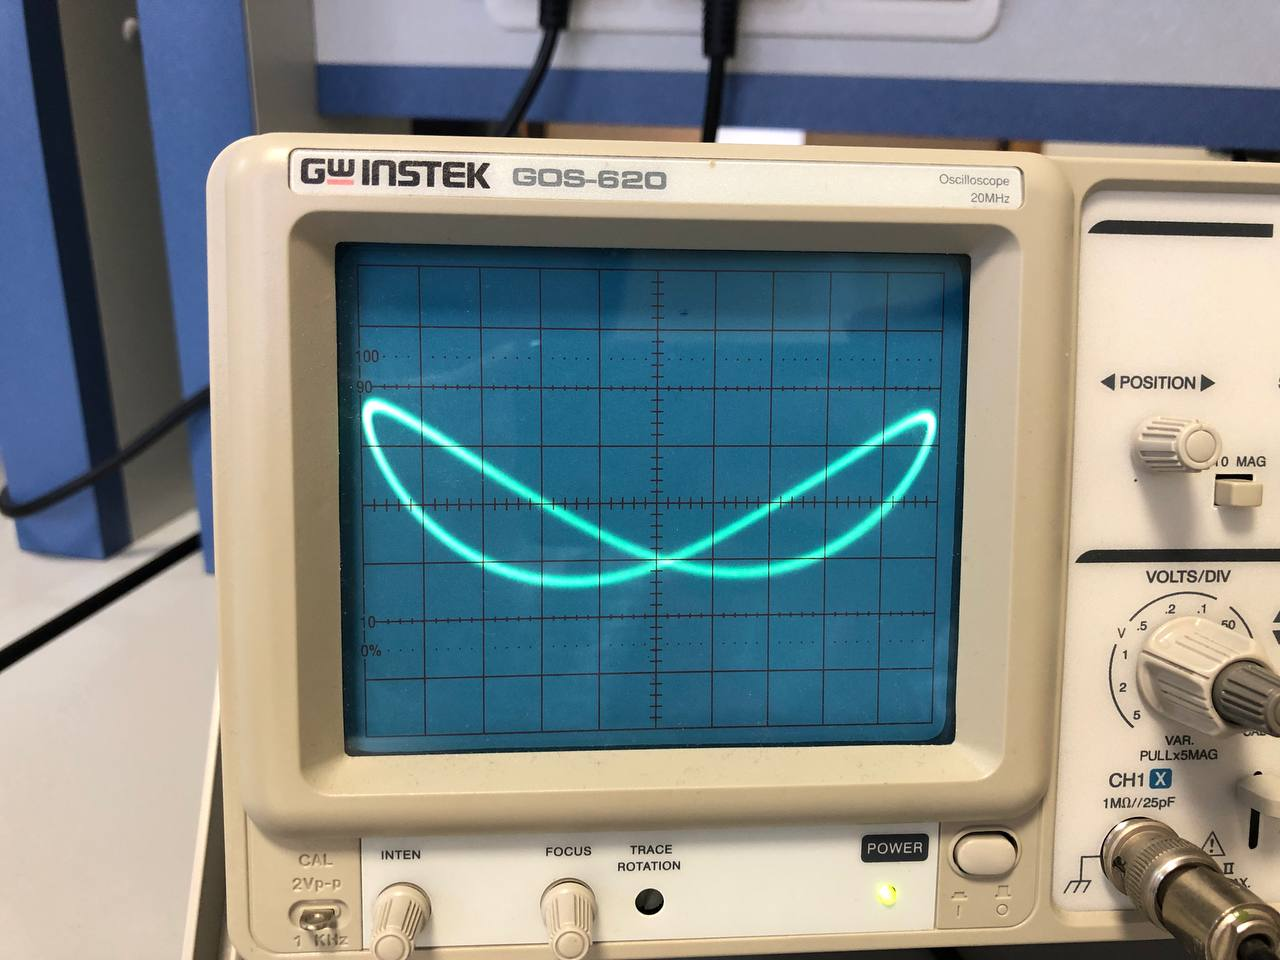
\includegraphics[width=0.8\linewidth]{img/fuck.jpg}
\end{figure}
